% Template for Cogsci submission with R Markdown

% Stuff changed from original Markdown PLOS Template
\documentclass[10pt, letterpaper]{article}

\usepackage{cogsci}
\usepackage{pslatex}
\usepackage{float}
\usepackage{caption}

% amsmath package, useful for mathematical formulas
\usepackage{amsmath}

% amssymb package, useful for mathematical symbols
\usepackage{amssymb}

% hyperref package, useful for hyperlinks
\usepackage{hyperref}

% graphicx package, useful for including eps and pdf graphics
% include graphics with the command \includegraphics
\usepackage{graphicx}

% Sweave(-like)
\usepackage{fancyvrb}
\DefineVerbatimEnvironment{Sinput}{Verbatim}{fontshape=sl}
\DefineVerbatimEnvironment{Soutput}{Verbatim}{}
\DefineVerbatimEnvironment{Scode}{Verbatim}{fontshape=sl}
\newenvironment{Schunk}{}{}
\DefineVerbatimEnvironment{Code}{Verbatim}{}
\DefineVerbatimEnvironment{CodeInput}{Verbatim}{fontshape=sl}
\DefineVerbatimEnvironment{CodeOutput}{Verbatim}{}
\newenvironment{CodeChunk}{}{}

% cite package, to clean up citations in the main text. Do not remove.
\usepackage{cite}

\usepackage{color}

% Use doublespacing - comment out for single spacing
%\usepackage{setspace}
%\doublespacing


% % Text layout
% \topmargin 0.0cm
% \oddsidemargin 0.5cm
% \evensidemargin 0.5cm
% \textwidth 16cm
% \textheight 21cm

\title{Developmental and postural changes in children's visual access to faces}


\author{{\large \bf Alessandro Sanchez} \\ \texttt{author1@university.edu} \\ Department of Psychology \\ Stanford University \And {\large \bf Bria Long} \\ \texttt{bria@stanford.edu} \\ Department of Psychology \\ Stanford University
    \And {\large \bf Ally Kraus} \\ \texttt{bria@stanford.edu} \\ Department of Psychology \\ Stanford University
    \And {\large \bf Michael C. Frank} \\ \texttt{mcfrank@stanford.edu} \\ Department of Psychology \\ Stanford University}

\begin{document}

\maketitle

\begin{abstract}


\textbf{Keywords:}
social cognition; face-perception; infancy; locomotion; head-cameras
\end{abstract}

\section{Methods}\label{methods}

\subsection{Participants}\label{participants}

Our final sample consisted of 36 infants and children, with 8
participants in three age groups: 8 months (6 females), 12 months (7
females), and 16 months (6 females). Participants were recruited from
the surrounding community via state birth records, had no documented
disabilities, and were reported to hear at least 80\% English at home.
Demographics and exclusion rates are given in Table \ref{tab:pop}.

\begin{table}[H]
\centering
\begin{tabular}{rrrrrr}
  \hline
 Group & N & \% incl. & Mean age & Videos length (min) \\ 
  \hline
   8 mo. &   12 & 0.46 & 8.71 & 14.41 \\ 
   12 mo. &  12 & 0.40 & 12.62 & 13.48 \\ 
   16 mo. &  12 & 0.31 & 16.29 & 15.00\\ 
   \hline
\end{tabular}
\caption{\label{tab:pop} Demographics by age group.}
\end{table}

To obtain this final sample, we tested 95, excluding 59 children for the
following reasons: 20 for technical issues related to the headcam, 15
for failing to wear the headcam, 10 for fewer than 4 minutes of headcam
footage, 5 for having multiple adults present, 5 for missing CDI data, 2
for missing scene camera footage, 1 for fussiness, and one excluded for
sample symmetry. All inclusion decisions were made independent of the
results of subsequent analyses.

\subsection{Head-mounted camera}\label{head-mounted-camera}

We used a small, head-mounted camera (``headcam'') that was constructed
from a MD80 model camera attached to a soft elastic headband.Videos
captured by the headcam were 720x480 pixels with 25 frames per
second.Detailed instructions for creating this headcam can be found at
\url{http://babieslearninglanguage.blogspot.com/2013/10/how-to-make-babycam.html}.
A fisheye lens was attached to the camera to cincrease the view angle
from \(32^{\circ}\) horizontal by \(24^{\circ}\) vertical to
\(64^{\circ}\) horizontal by \(46^{\circ}\) vertical (see Figure
\ref{fig:headcam}, left).

Even with the fish-eye lens, the vertical field of view of the camera is
still considerably reduced compared to the child's approximate vertical
field of view, which spans around 100--120\(^{\circ}\) in the vertical
dimension by 6-7 months of age (Cummings, Van Hof-Van Duin, Mayer,
Hansen, \& Fulton, 1988; Mayer, Fulton, \& Cummings, 1988). As we were
primarily interested in the presence of faces in the child's field of
view, we chose to orient the camera upwards to capture the entirely of
the child's upper visual field where the child is likely to see the
faces of adults around them. This allowed us to maximize our chances of
capturing faces that the child would have seen during the play session.

\begin{CodeChunk}
\begin{figure}[H]

{\centering 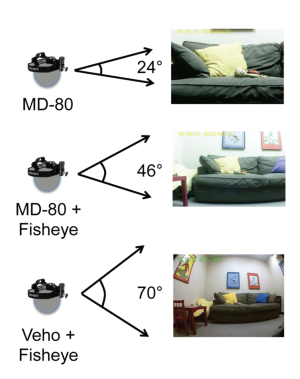
\includegraphics{figs/image-1} 

}

\caption[Field of view for three different headcam configurations, with the device we used in the middle]{Field of view for three different headcam configurations, with the device we used in the middle. The lowest camera is pictured for comparison, but was not available until after our study was already in progress.}\label{fig:image}
\end{figure}
\end{CodeChunk}

\subsection{Procedure}\label{procedure}

First, all parents signed consent documentsin a waiting room where
children were fitted with the headcam. After the child was comfortable
in the waiting room and with the experimenter, the experimenter placed
the headcam on the child's head. If the child was uninterested in
wearing the headcam or tried to take it off, the experimenter presented
engaging toys to try to draw the child's focus away from the headcam
(Yoshida \& Smith, 2008).

After the child was comfortable with wearing the headcam, the child and
caregiver were shown to a playroom for the free-play session--the focus
of the current study. Parents were shown a box containing three pairs of
novel and familiar objects (e.g., a ball and a feather duster, named a
``zem''), and were instructed to play with the object pairs with their
child one at a time, ``as they typically would.'' All parents confirmed
that their child had not previosuly seen the novel toys and were
instructed to use the novel labels to refer to the novel toys.

The experimenter then left the playroom for approximately 15 minutes,
during which a tripod-mounted camera in the corner of the room recorded
the session and the headcam captured video from the child's perspective.

\subsection{Data Processing and
Annotation}\label{data-processing-and-annotation}

\begin{figure*}
\includegraphics[width=6in]{images/framesample.pdf}
\caption{\label{fig:frames} Sample frames from the headcam videos for a child from each age group, selected because they featured successful face detections (green squares).}
\end{figure*}

All headcam videos were cropped to exclude the period of entry to the
playroom and were automatically synchronized with the tripod-mounted
videos using FinalCut Pro Software. These sessions yielded a substantial
amount of video: a total of 516 minutes (almost a milion frames), with
an average video length of 8.6 minutes (min = 4.53, max = 19.35).

\subsubsection{Posture and Orientation
Annotation}\label{posture-and-orientation-annotation}

We created a set of custom annotations that described the child's
physical posture (e.g.~standing) and the orientation of the caregiver
relative to the child (e.g.~far away). The child's posture was
categorized as being held/carried, prone (crawling or lying), sitting,
or standing. The caregiver's orientation was characterized as being
close to the child, farther from the child, and a global category of
caregiver behind the child. For the first two annotationes (close/far
from the child), the caregiver could either be to the the front or to
the side of the child. All annontations were made using
OpenSHAPA/Datavyu software (Adolph, Gilmore, Freeman, Sanderson, \&
Millman, 2012), and times when the child was out of view of the tripod
camera was marked as uncodable and was excluded from these annotations.

\subsection{Face Detection}\label{face-detection}

An additional goal of the study was to measure the presence of
caregivers' faces in the child's field of view (as approximated by the
headcam). To avoid hand-annotating the size and position of faces in
every frame of video, we tested two face detection systems. Sample
frames from the video with successful detections are given in Figure
\ref{fig:frames}.

\subsubsection{Face detection
algorithms}\label{face-detection-algorithms}

\subsubsection{Detector evaluation}\label{detector-evaluation}

\begin{table}[t]
  \caption{Model performance on gold standard generalization training set dataset. P, R, and F denote precision, recall, and F-score for each of the two samples. \label{tab:model_eval}}
  \begin{center}
    \begin{tabular}{l|ccc|ccc}
      \hline
       &  \multicolumn{3}{c|}{High-density} &  \multicolumn{3}{c}{Random} \\
      % \null Model & P & R & F & P & R & F  \\
      \hline
      % Viola-Jones & .55  & .38 &  .45 & .89 & .74 & .81   \\
      % MTCNN & .86 & .78 & .81 & .93 & .76 & .83 \\
      % OpenPose & .86 & .78 & .81 & .93 & .76 & .83 \\
    \hline
    \end{tabular}
  \end{center}
\end{table}

\section{Results}\label{results}

We report results from three different sets of analyses. First, we
explore developmental changes in posture and orientation in our dataset.
Next, we explore how these changes affect access to faces and to hands,
as measured using computater vision algorithms. Finally, we explore how
these changes impact the accessibility of faces and hands during
labeling events.

\subsection{Changes in Posture and
Orientation}\label{changes-in-posture-and-orientation}

\subsection{Changes in Access to
Faces}\label{changes-in-access-to-faces}

\subsection{Changes in Access to
Hands}\label{changes-in-access-to-hands}

\section{Acknowledgements}\label{acknowledgements}

Thanks to Kaia Simmons, Kathy Woo, Aditi Maliwal, and other members of
the Language and Cognition Lab for help in recruitment, data collection,
and annotation. This research was supported by a John Merck Scholars
grant to MCF. An earlier version of this work was presented to the
Cognitive Science Society in Frank, Simmons, Yurovsky, \& Pusiol (2013).
Please address correspondence to Michael C. Frank, Department of
Psychology, Stanford University, 450 Serra Mall (Jordan Hall), Stanford,
CA, 94305, tel: (650) 724-4003, email: \texttt{mcfrank@stanford.edu}.

\section{References}\label{references}

\setlength{\parindent}{-0.1in} \setlength{\leftskip}{0.125in} \noindent

\hypertarget{refs}{}
\hypertarget{ref-adolph2012}{}
Adolph, K., Gilmore, R., Freeman, C., Sanderson, P., \& Millman, D.
(2012). Toward open behavioral science. \emph{Psychological Inquiry},
\emph{23}(3), 244--247.

\hypertarget{ref-cummings1988}{}
Cummings, M., Van Hof-Van Duin, J., Mayer, D., Hansen, R., \& Fulton, A.
(1988). Visual fields of young children. \emph{Behavioural and Brain
Research}, \emph{29}(1), 7--16.

\hypertarget{ref-frank2013}{}
Frank, M. C., Simmons, K., Yurovsky, D., \& Pusiol, G. (2013).
Developmental and postural changes in children’s visual access to faces.
In \emph{Proceedings of the 35th annual meeting of the cognitive science
society} (pp. 454--459).

\hypertarget{ref-mayer1988}{}
Mayer, D., Fulton, A., \& Cummings, M. (1988). Visual fields of infants
assessed with a new perimetric technique. \emph{Investigative
Ophthalmology \& Visual Science}, \emph{29}(3), 452--459.

\hypertarget{ref-yoshida2008}{}
Yoshida, H., \& Smith, L. (2008). What's in view for toddlers? Using a
head camera to study visual experience. \emph{Infancy}, \emph{13},
229--248.

\end{document}
